\documentclass[twoside]{book}

% Packages required by doxygen
\usepackage{fixltx2e}
\usepackage{calc}
\usepackage{doxygen}
\usepackage[export]{adjustbox} % also loads graphicx
\usepackage{graphicx}
\usepackage[utf8]{inputenc}
\usepackage{makeidx}
\usepackage{multicol}
\usepackage{multirow}
\PassOptionsToPackage{warn}{textcomp}
\usepackage{textcomp}
\usepackage[nointegrals]{wasysym}
\usepackage[table]{xcolor}

% NLS support packages
\usepackage[ngerman]{babel}

% Font selection
\usepackage[T1]{fontenc}
\usepackage[scaled=.90]{helvet}
\usepackage{courier}
\usepackage{amssymb}
\usepackage{sectsty}
\renewcommand{\familydefault}{\sfdefault}
\allsectionsfont{%
  \fontseries{bc}\selectfont%
  \color{darkgray}%
}
\renewcommand{\DoxyLabelFont}{%
  \fontseries{bc}\selectfont%
  \color{darkgray}%
}
\newcommand{\+}{\discretionary{\mbox{\scriptsize$\hookleftarrow$}}{}{}}

% Page & text layout
\usepackage{geometry}
\geometry{%
  a4paper,%
  top=2.5cm,%
  bottom=2.5cm,%
  left=2.5cm,%
  right=2.5cm%
}
\tolerance=750
\hfuzz=15pt
\hbadness=750
\setlength{\emergencystretch}{15pt}
\setlength{\parindent}{0cm}
\setlength{\parskip}{3ex plus 2ex minus 2ex}
\makeatletter
\renewcommand{\paragraph}{%
  \@startsection{paragraph}{4}{0ex}{-1.0ex}{1.0ex}{%
    \normalfont\normalsize\bfseries\SS@parafont%
  }%
}
\renewcommand{\subparagraph}{%
  \@startsection{subparagraph}{5}{0ex}{-1.0ex}{1.0ex}{%
    \normalfont\normalsize\bfseries\SS@subparafont%
  }%
}
\makeatother

% Headers & footers
\usepackage{fancyhdr}
\pagestyle{fancyplain}
\fancyhead[LE]{\fancyplain{}{\bfseries\thepage}}
\fancyhead[CE]{\fancyplain{}{}}
\fancyhead[RE]{\fancyplain{}{\bfseries\leftmark}}
\fancyhead[LO]{\fancyplain{}{\bfseries\rightmark}}
\fancyhead[CO]{\fancyplain{}{}}
\fancyhead[RO]{\fancyplain{}{\bfseries\thepage}}
\fancyfoot[LE]{\fancyplain{}{}}
\fancyfoot[CE]{\fancyplain{}{}}
\fancyfoot[RE]{\fancyplain{}{\bfseries\scriptsize Erzeugt von Doxygen }}
\fancyfoot[LO]{\fancyplain{}{\bfseries\scriptsize Erzeugt von Doxygen }}
\fancyfoot[CO]{\fancyplain{}{}}
\fancyfoot[RO]{\fancyplain{}{}}
\renewcommand{\footrulewidth}{0.4pt}
\renewcommand{\chaptermark}[1]{%
  \markboth{#1}{}%
}
\renewcommand{\sectionmark}[1]{%
  \markright{\thesection\ #1}%
}

% Indices & bibliography
\usepackage{natbib}
\usepackage[titles]{tocloft}
\setcounter{tocdepth}{3}
\setcounter{secnumdepth}{5}
\makeindex

% Hyperlinks (required, but should be loaded last)
\usepackage{ifpdf}
\ifpdf
  \usepackage[pdftex,pagebackref=true]{hyperref}
\else
  \usepackage[ps2pdf,pagebackref=true]{hyperref}
\fi
\hypersetup{%
  colorlinks=true,%
  linkcolor=blue,%
  citecolor=blue,%
  unicode%
}

% Custom commands
\newcommand{\clearemptydoublepage}{%
  \newpage{\pagestyle{empty}\cleardoublepage}%
}

\usepackage{caption}
\captionsetup{labelsep=space,justification=centering,font={bf},singlelinecheck=off,skip=4pt,position=top}

%===== C O N T E N T S =====

\begin{document}

% Titlepage & ToC
\hypersetup{pageanchor=false,
             bookmarksnumbered=true,
             pdfencoding=unicode
            }
\pagenumbering{alph}
\begin{titlepage}
\vspace*{7cm}
\begin{center}%
{\Large Spannungsteiler }\\
\vspace*{1cm}
{\large Erzeugt von Doxygen 1.8.13}\\
\end{center}
\end{titlepage}
\clearemptydoublepage
\pagenumbering{roman}
\tableofcontents
\clearemptydoublepage
\pagenumbering{arabic}
\hypersetup{pageanchor=true}

%--- Begin generated contents ---
\chapter{P\+M\+Sw\+Eng -\/ Projektmanagement und Software Engeneering}
\label{index}\hypertarget{index}{}In diesem Programm kann die Spannungen u1 und u2 für einen Spannungsteiler eingeben, das Programm berechnet die best mögliche Kombination von zwei Widerstände.

\subsection*{Ersteller des Projektes}


\begin{DoxyItemize}
\item Samuel Schuler
\item Sven Suter
\item Francisco Stocker
\item Christian Dieterle 
\end{DoxyItemize}
\chapter{Hierarchie-\/\+Verzeichnis}
\section{Klassenhierarchie}
Die Liste der Ableitungen ist -\/mit Einschränkungen-\/ alphabetisch sortiert\+:\begin{DoxyCompactList}
\item Q\+Main\+Window\begin{DoxyCompactList}
\item \contentsline{section}{Main\+Window}{\pageref{classMainWindow}}{}
\end{DoxyCompactList}
\end{DoxyCompactList}

\chapter{Klassen-\/\+Verzeichnis}
\section{Auflistung der Klassen}
Hier folgt die Aufzählung aller Klassen, Strukturen, Varianten und Schnittstellen mit einer Kurzbeschreibung\+:\begin{DoxyCompactList}
\item\contentsline{section}{\hyperlink{classMainWindow}{Main\+Window} }{\pageref{classMainWindow}}{}
\end{DoxyCompactList}

\chapter{Klassen-\/\+Dokumentation}
\hypertarget{classMainWindow}{}\section{Main\+Window Klassenreferenz}
\label{classMainWindow}\index{Main\+Window@{Main\+Window}}


Klassendiagramm für Main\+Window\+:\nopagebreak
\begin{figure}[H]
\begin{center}
\leavevmode
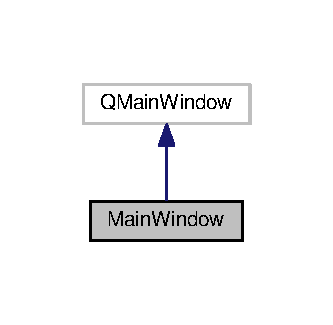
\includegraphics[width=160pt]{classMainWindow__inherit__graph}
\end{center}
\end{figure}
\subsection*{Öffentliche Methoden}
\begin{DoxyCompactItemize}
\item 
{\bfseries Main\+Window} (Q\+Widget $\ast$parent=nullptr)\hypertarget{classMainWindow_a996c5a2b6f77944776856f08ec30858d}{}\label{classMainWindow_a996c5a2b6f77944776856f08ec30858d}

\item 
void \hyperlink{classMainWindow_a2928be63df3071466644eca76d6e32a7}{start\+Calculation} ()\hypertarget{classMainWindow_a2928be63df3071466644eca76d6e32a7}{}\label{classMainWindow_a2928be63df3071466644eca76d6e32a7}

\begin{DoxyCompactList}\small\item\em Wird aufgerufen wenn der berechnen Button angeklickt wird. Damit wird der ganze Ablauf für eine Widerstandsberchnung gestartet. \end{DoxyCompactList}\item 
int \hyperlink{classMainWindow_a3b94ad2c855f6a0df3579c48b1a6f6fd}{read\+U1} ()
\begin{DoxyCompactList}\small\item\em Liest die Spannung U1 vom Eingabefeld. \end{DoxyCompactList}\item 
int \hyperlink{classMainWindow_ab9a4bb81031d0bcb5cc5d181a26f3429}{read\+U2} ()
\begin{DoxyCompactList}\small\item\em Liest die Spannung U2 vom Eingabefeld. \end{DoxyCompactList}\item 
int \hyperlink{classMainWindow_a4869d3468f1124ae508be8e177b66ed3}{read\+Reihe} ()
\begin{DoxyCompactList}\small\item\em Schaut welche E-\/\+Reihe im G\+UI ausgewählt wurde. \end{DoxyCompactList}\item 
void {\bfseries output\+Values} (double r1, double r2, int fail)\hypertarget{classMainWindow_a12b9bbad12422386cec9da99c2ea3d57}{}\label{classMainWindow_a12b9bbad12422386cec9da99c2ea3d57}

\item 
int {\bfseries calculate} (int u1, int u2, int reihe)\hypertarget{classMainWindow_ab0f78571621e4f8e82f51464648cf017}{}\label{classMainWindow_ab0f78571621e4f8e82f51464648cf017}

\end{DoxyCompactItemize}


\subsection{Dokumentation der Elementfunktionen}
\index{Main\+Window@{Main\+Window}!read\+Reihe@{read\+Reihe}}
\index{read\+Reihe@{read\+Reihe}!Main\+Window@{Main\+Window}}
\subsubsection[{\texorpdfstring{read\+Reihe()}{readReihe()}}]{\setlength{\rightskip}{0pt plus 5cm}int Main\+Window\+::read\+Reihe (
\begin{DoxyParamCaption}
{}
\end{DoxyParamCaption}
)}\hypertarget{classMainWindow_a4869d3468f1124ae508be8e177b66ed3}{}\label{classMainWindow_a4869d3468f1124ae508be8e177b66ed3}


Schaut welche E-\/\+Reihe im G\+UI ausgewählt wurde. 

\begin{DoxyReturn}{Rückgabe}
Gibt die ausgewählte E-\/\+Reihe zurück. (enum\+: E3, E6, E12, E24) 
\end{DoxyReturn}
\index{Main\+Window@{Main\+Window}!read\+U1@{read\+U1}}
\index{read\+U1@{read\+U1}!Main\+Window@{Main\+Window}}
\subsubsection[{\texorpdfstring{read\+U1()}{readU1()}}]{\setlength{\rightskip}{0pt plus 5cm}int Main\+Window\+::read\+U1 (
\begin{DoxyParamCaption}
{}
\end{DoxyParamCaption}
)}\hypertarget{classMainWindow_a3b94ad2c855f6a0df3579c48b1a6f6fd}{}\label{classMainWindow_a3b94ad2c855f6a0df3579c48b1a6f6fd}


Liest die Spannung U1 vom Eingabefeld. 

\begin{DoxyReturn}{Rückgabe}
Gibt die Spannung in uV zurück. 
\end{DoxyReturn}
\index{Main\+Window@{Main\+Window}!read\+U2@{read\+U2}}
\index{read\+U2@{read\+U2}!Main\+Window@{Main\+Window}}
\subsubsection[{\texorpdfstring{read\+U2()}{readU2()}}]{\setlength{\rightskip}{0pt plus 5cm}int Main\+Window\+::read\+U2 (
\begin{DoxyParamCaption}
{}
\end{DoxyParamCaption}
)}\hypertarget{classMainWindow_ab9a4bb81031d0bcb5cc5d181a26f3429}{}\label{classMainWindow_ab9a4bb81031d0bcb5cc5d181a26f3429}


Liest die Spannung U2 vom Eingabefeld. 

\begin{DoxyReturn}{Rückgabe}
Gibt die Spannung in uV zurück. 
\end{DoxyReturn}


Die Dokumentation für diese Klasse wurde erzeugt aufgrund der Dateien\+:\begin{DoxyCompactItemize}
\item 
Main\+Window.\+h\item 
Main\+Window.\+cpp\end{DoxyCompactItemize}

%--- End generated contents ---

% Index
\backmatter
\newpage
\phantomsection
\clearemptydoublepage
\addcontentsline{toc}{chapter}{Index}
\printindex

\end{document}
